\chapter{Evaluation}

Dieses Kapitel bewertet die praktische Nutzbarkeit der implementierten VirtIO-Treiberint\-egration in drei Dimensionen: (i) funktionale Verifikation der VirGL-Erweiterung über einen Smoke Test, (ii) funktionaler Nachweis der Audioausgabe über VirtIO-Sound anhand eines PCM-Playback-Tests und (iii) quantitative Leistungsbewertung der Grafikpipeline anhand der Rectangle-Demo. Die Messlogik der Demo orientiert sich am in der Vorarbeit etablierten Vorgehen, bei dem Frames gezählt und die verstrichene Zeit über \code{sys\_get\_system\_time()} bestimmt wird.\\
\\
Alle Demos werden dabei aus der \code{boot.rs} Datei heraus mit den Funktionsaufrufen \code{test\_virgl()}, \code{play\_pcm\_file()} und \code{rectangle\_demo()} gestartet.

\section{Ausgabe des VirGL Smoke Tests}

Der VirGL Smoke Test \code{test\_virgl} dient als End-to-End-Nachweis dafür, dass der 3D-Command-Stream vom Host akzeptiert und verarbeitet wird. Der Test durchläuft dabei die in Kapitel 4.2 beschriebenen Schritte (Kontext erzeugen, 3D-Resource erstellen, Command Stream submitten, Darstellung über Flush).

Zur Dokumentation werden die wichtigsten Debug-Ausgaben herangezogen, die die erfolgreiche Abarbeitung der einzelnen Etappen zeigen. Die folgende Terminalausgabe enthält einen gekürzten Log-Auszug.

\begin{terminalblock}
  \begin{textcode}
[0.274][INF][gpu.rs@904] Starting Virgl 3D test...
virtio_gpu_cmd_ctx_create ctx 0x1, name test_ctx
virtio_gpu_cmd_get_display_info
virtio_gpu_cmd_res_create_3d res 0x2000, fmt 0x1, w 640, h 480, d 1
virtio_gpu_cmd_ctx_res_attach ctx 0x1, res 0x2000
virtio_gpu_cmd_set_scanout id 0, res 0x2000, w 640, h 480, x 0, y 0
...
Sende 108 Bytes an 3D-Befehlen...
virtio_gpu_cmd_ctx_submit ctx 0x1, size 108
virtio_gpu_fence_ctrl fence 0x1, type 0x207
virtio_gpu_fence_resp fence 0x1
ctx_submit rsp type=0x1100, fence_id=0x1, ctx=0x1
virtio_gpu_cmd_res_flush res 0x2000, w 640, h 480, x 0, y 0
[0.361][INF][gpu.rs@973] Rendered green frame and displayed successfully!
  \end{textcode}
\end{terminalblock}

Die Ausgaben zeigen, dass (i) der 3D-Kontext erstellt wird, (ii) die 3D-Resource angelegt und an den Kontext gebunden wird, (iii) der Command-Stream mit \code{CMD\_SUBMIT\_3D} übertragen wird und (iv) der Host eine Fence-Antwort liefert. Letzteres ist ein Indikator dafür, dass die Submission verarbeitet wurde und auf einer Synchronisations-Timeline eindeutig referenzierbar ist.

Zusätzlich lässt sich die korrekte Kodierung des Command-Streams direkt über die Debug-Ausgabe der Funktion \code{dump\_cs} nachvollziehen. Dabei werden die im Command-Stream enthaltenen 32-Bit Headerwörter dekodiert und als Tripel \code{(cmd, obj, len)} ausgegeben. Die Dekodierung folgt der in Abschnitt 4.2 beschriebenen Bitaufteilung, wobei \code{cmd} die unteren 8 Bit, \code{obj} die nächsten 8 Bit und \code{len} die oberen 16 Bit (Anzahl der folgenden 32-Bit Payload-Wörter) repräsentiert:

\begin{codeblock}{gpu.rs}{Rust}
  \begin{rustcode}
fn decode_hdr(h: u32) -> (u32,u32,u32) {
    let cmd =  h        & 0xff;
    let obj = (h >> 8)  & 0xff;
    let len =  h >> 16;
    (cmd, obj, len)
}
  \end{rustcode}
\end{codeblock}

Im Log des Smoke Tests erscheinen dadurch die folgenden dekodierten Header:

\begin{itemize}
	\item \code{hdr @000: cmd=1 obj=8 len=5}
	\item \code{hdr @024: cmd=5 obj=0 len=3}
	\item \code{hdr @040: cmd=4 obj=0 len=7}
	\item \code{hdr @072: cmd=7 obj=0 len=8}
\end{itemize}

Diese Werte stimmen mit der erwarteten Encodierung der verwendeten Encoder überein. So beginnt etwa \code{encode\_create\_surface} mit einem Headerwort, das über \code{virgl\_cmd0(}\\ \code{VIRGL\_CCMD\_CREATE\_OBJECT, VIRGL\_OBJECT\_SURFACE, 5)} erzeugt wird. Die Wertezuordnung erfolgt direkt: \code{VIRGL\_CCMD\_CREATE\_OBJECT = 1} steht dabei für das Kommando \code{cmd=1}. Analog dazu entspricht \code{VIRGL\_OBJECT\_SURFACE = 8} dem Objekt \code{obj=8}. Der Parameter \code{len=5} beschreibt schließlich die nachfolgenden fünf 32-Bit Payload-Wörter des Encoders. Die Dump-Ausgabe liefert damit einen zusätzlichen, internen Konsistenznachweis dafür, dass der erzeugte Byte-Stream strukturell korrekt aufgebaut ist und vom Host in dieser Struktur verarbeitet werden kann.\\
\\
Abschließend liefert das visuelle Ergebnis den entscheidenden funktionalen Nachweis für die korrekte Interpretation der Befehlskette. Wie bereits in Abschnitt 4.2 hergeleitet, definieren die im Testcode über \code{encode\_clear\_color} gesetzten normalisierten Fließkommawerte ($R=0.094$, $G=0.416$, $B=0.067$, $A=1.0$) nach der Skalierung in den 8-Bit-Farbraum die RGBA-Farbe $(24, 106, 17, 255)$.\\
\\
Der in Abbildung 5.1 dargestellte Framebuffer zeigt exakt diese dunkelgrüne Färbung. Da diese Farbinformation ausschließlich über den 3D-Befehl \code{VIRGL\_CCMD\_CLEAR} im Command"=Stream übermittelt wurde, beweist die korrekte Darstellung, dass die gesamte Pipeline von der Submission im Gast über die Verarbeitung im Host bis zum Flush funktional intakt ist.

\begin{figure}[H]
  \centering
  \begin{subfigure}[b]{0.5\textwidth}
    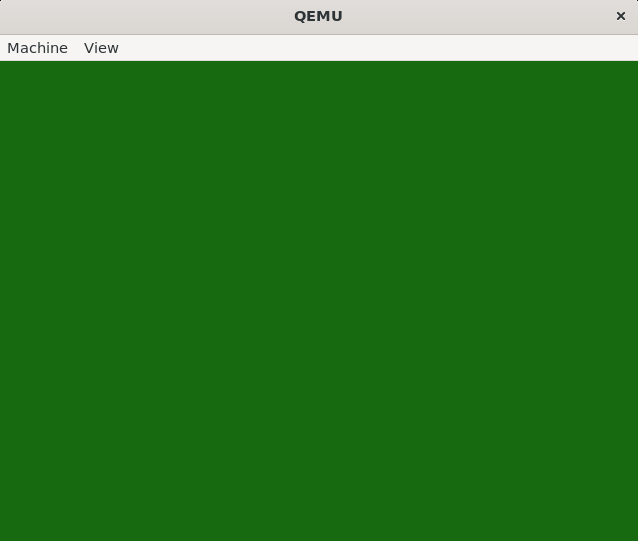
\includegraphics[width=1.0\linewidth]{img/qemuvirglgreen}
  \end{subfigure}
  \caption{Screenshot des VirGL Smoke Tests\\
  (R = 24, G = 106, B= 17, A = 255)}
  \label{grafik_2}
\end{figure}

\clearpage

\section{VirtIO-Sound (PCM-Playback)}

Zur Validierung der VirtIO-Sound-Anbindung wurde die Beispielroutine ausgeführt. Der Test bettet eine PCM-Datei direkt in das Kernel-Image ein und konfiguriert anschließend den ersten verfügbaren Output-Stream des VirtIO-Sound-Geräts. Die Ausgabe erfolgt blockweise in periodengroßen Transfers, wobei mehrere Perioden gleichzeitig in der TX-Queue gehalten werden, um eine kontinuierliche Wiedergabe sicherzustellen und Unterläufe zu vermeiden.\\

Im Log ist zunächst erkennbar, dass die PCM-Fähigkeiten des Geräts erfolgreich abgefragt werden. Für den Output-Stream werden dabei u. a. eine breite Menge unterstützter Abtastraten bis hin zu 384 kHz sowie mehrere Sampleformate (S8/U8, S16/U16, S32/U32, Float) ausgegeben. Anschließend werden die Zielparameter für den Test festgelegt und protokolliert: \code{rate=44100}, \code{fmt=S16}, \code{ch=2}, \code{period=4096 B} und \code{buffer=32768 B}

Während der Initialisierung tritt einmalig die Warnung „Error getting chmap infos“ auf. Diese Warnung betrifft die Abfrage der Channel-Map (Zuordnung der Kanäle, z. B. links/rechts). Für den vorliegenden Stereo-Test (\code{ch=2}) ist diese Information nicht zwingend erforderlich, da die Wiedergabe mit Standardzuordnung erfolgt und die PCM-Konfiguration sowie der Streamstart erfolgreich sind. Entscheidend ist, dass die Playback-Pipeline anschließend vollständig durchläuft und die Wiedergabe mit „PCM file playback finished“ abgeschlossen wird.

\begin{terminalblock}
  \begin{textcode}
[0.125][INF][sound.rs@192] [sound device] pcm_info: features: PcmFeatures(0x0), rates: PcmRates(RATE_5512 | RATE_8000 | RATE_11025 | RATE_16000 | RATE_22050 | RATE_32000 | RATE_44100 | RATE_48000 | RATE_64000 | RATE_88200 | RATE_96000 | RATE_176400 | RATE_192000 | RATE_384000), formats: PcmFormats(S8 | U8 | S16 | U16 | S32 | U32 | FLOAT), direction: OUTPUT
[0.127][INF][sound.rs@192] [sound device] pcm_info: features: PcmFeatures(0x0), rates: PcmRates(RATE_5512 | RATE_8000 | RATE_11025 | RATE_16000 | RATE_22050 | RATE_32000 | RATE_44100 | RATE_48000 | RATE_64000 | RATE_88200 | RATE_96000 | RATE_176400 | RATE_192000 | RATE_384000), formats: PcmFormats(S8 | U8 | S16 | U16 | S32 | U32 | FLOAT), direction: INPUT
[0.128][WRN][sound.rs@204] [sound device] Error getting chmap infos
[0.129][INF][virtio_tests.rs@094] PCM config -> rate=Rate44100, fmt=S16, ch=2, period=4096 B, buffer=32768 B
[231.930][INF][virtio_tests.rs@154] PCM file playback finished
  \end{textcode}
\end{terminalblock}

Zusätzlich lässt sich über die Zeitstempel der Logausgaben die Dauer des Tests abschätzen: Zwischen der Konfigurationsausgabe bei ca. 0.129\,s und dem Abschluss bei 231.930\,s liegen rund 231.8\,s ($\approx$ 3 min 52\,s). Dies entspricht der Länge der verwendeten Audiodatei (3:52 Minuten, Taylor Swift – Blank Space (Lyrics)\cite{YoutubeBlankSpace}) und zeigt damit, dass der Stream über die gesamte Laufzeit stabil bedient werden konnte. Insgesamt belegt der Test die End-to-End-Funktionalität des Datenpfads vom Gast (Virtqueue-Transfers) über den Hypervisor bis zur Host-Audiokette.

\clearpage

\section{Leistung: Rectangle-Demo}

Die Rectangle-Demo erzeugt eine konstante Renderlast, indem eine feste Anzahl farbiger Rechtecke (hier: 500 Rechtecke) kontinuierlich über den Bildschirm bewegt und pro Frame neu gerendert wird. Die FPS-Ermittlung erfolgt über Framezählung und Zeitmessung in festen Intervallen, analog zur in der Vorarbeit beschriebenen Messlogik.

Die Demo wurde für unterschiedliche Umgebungen und Auflösungen ausgeführt, wobei folgende Hardware-Konfiguration verwendet wurde:

\begin{itemize}
    \item CPU: AMD Ryzen 7 3700x (8 Kerne, 4.20 GHz)
    \item GPU: AMD Radeon RX 7900 XT
	\item Host-Umgebung A: Ubuntu 25.10
	\item Host-Umgebung B: WSL2 (Ubuntu 24.04.1 LTS)
	\item Drei Auflösungen: 640x480, 1920×1080, 2560x1440
\end{itemize}

Jeder Testlauf wurde über 3 Minuten ausgeführt, wodurch pro Konfiguration mehrere 30-Sekunden-Messpunkte entstehen.

\subsection{Messmethodik und Korrektur der Zeitbasis}

Die Demo berechnet FPS als Quotient aus gerenderten Frames und verstrichener Zeit. In der Referenzimplementierung wird hierfür \code{sys\_get\_system\_time()} verwendet, und es wird in regelmäßigen Intervallen (alle 30 Sekunden) geloggt.

In der hier betrachteten Implementierung werden bestimmte GPU-Zugriffe in kurzen kritischen Abschnitten ausgeführt, die Interrupts temporär deaktivieren (zur Vermeidung von „Interrupt Storms“ durch Demo-Thread und VirtIO-Interruptpfad). Da D3OS die Systemzeit Timer-Interrupt fortschreibt, bleibt \code{sys\_get\_system\_time()} während interruptfreier Abschnitte stehen. Dadurch kann es zu einer Abweichung zwischen „Gastzeit“ und tatsächlich verstrichener Hostzeit kommen, was eine direkte FPS-Auswertung auf Basis der Gastzeit verfälschen würde.

Um die reale Bildrate zu bestimmen, wird daher pro 30-Sekunden-Messintervall zusätzlich die tatsächlich auf dem Host verstrichene Zeit $t_{\mathrm{host}}$ erfasst. Aus dem im Gast geloggten FPS-Wert $\mathrm{FPS}_{\mathrm{guest}}$ und der Gastintervalllänge $t_{\mathrm{guest}} = 30$\,s ergibt sich zunächst die Frameanzahl:
\[
N_{\mathrm{frames}} = \mathrm{FPS}_{\mathrm{guest}} \cdot t_{\mathrm{guest}}
\]
Die korrigierte, reale Bildrate berechnet sich anschließend als:
\[
\mathrm{FPS}_{\mathrm{real}} = \frac{N_{\mathrm{frames}}}{t_{\mathrm{host}}}
\]
Beispielrechnung: Bei $\mathrm{FPS}_{\mathrm{guest}} = 998$\,$\mathrm{fps}$ über $t_{\mathrm{guest}} = 30$\,s entstehen $N_{\mathrm{frames}} = 998\,\mathrm{fps} \cdot 30\,\mathrm{s} = 29940$\,Frames. Wenn dafür auf dem Host $t_{\mathrm{host}} = 39$\,s vergehen, ergibt sich $\mathrm{FPS}_{\mathrm{real}} = \frac{29940}{39\,\mathrm{s}} \approx 768$\,fps.\\

Diese Korrektur wird für alle Messpunkte angewandt, bevor Mittelwerte pro Auflösung/Umgebung gebildet werden.

\clearpage

\subsection{Ergebnisse}

Die Messergebnisse werden pro Umgebung und Auflösung tabellarisch dargestellt. Die Tabellen zeigen dabei auch die jeweilige gemessene Zeitabweichung ($t_{\mathrm{drift}}$), welche sich aus der real verstrichen Host-Zeit $t_{\mathrm{host}}$ und konstanter Messdauer $t_{\mathrm{guest}}$ ergibt. Diese Zeitabweichung beschreibt also effektiv die Dauer, in der die CPU durch synchrone GPU-Operation blockiert war. Die korrigierten FPS-Werte ergeben sich aus der zuvor gezeigten Rechnung.

\begin{table}[H]
\begin{center}
    \begin{tabular}{| l | l | l | l | l | l |}
    \hline
    Umgebung & Auflösung & $t_{\mathrm{host}}$ & $t_{\mathrm{drift}}$ & $\mathrm{FPS}_{\mathrm{guest}}$ & $\mathrm{FPS}_{\mathrm{real}}$ \\ \hline
    Ubuntu25 & 640x480 & 30\,s & 0\,s & 5451 & 5451 \\ \hline
    Ubuntu25 & 1920x1080 & 32\,s & 2\,s & 997 & 935 \\ \hline
    Ubuntu25 & 2560x1440 & 39\,s & 9\,s & 998 & 768 \\ \hline
    \end{tabular}
\end{center}
\caption{Durchschnittliche FPS mit Ubuntu25 Host}
\label{tabelle_avarage_time}
\end{table}

Die Ergebnisse unter der nativen Linux-Host-Umgebung (Tabelle 5.1) demonstrieren eine hohe Effizienz bei der Verarbeitung der Grafikbefehle. Bei der Basisauflösung von 640x480 ist die Zeitabweichung nicht messbar ($0$\,s), was auf einen vernachlässigbaren Overhead der Grafikpipeline hindeutet und extrem hohe Bildraten ermöglicht. Mit steigender Auflösung und dem damit verbundenen höheren Datendurchsatz (Framebuffer-Größe) wächst die Zeitabweichung moderat an. Bei WQHD (2560x1440) beträgt der „Blindflug“ des Gastsystems 9\,s, was einer Blockierungszeit von ca. 23\,\% entspricht.\\

Im Kontrast dazu zeigt die Ausführung unter WSL2 (Tabelle 5.2) ein signifikant abweichendes Verhalten, das auf die strukturellen Unterschiede der Virtualisierungsarchitektur schließen lässt.

\begin{table}[H]
\begin{center}
    \begin{tabular}{| l | l | l | l | l | l |}
    \hline
    Umgebung & Auflösung & $t_{host}$ & $t_{drift}$ & $\mathrm{FPS}_{guest}$ & $\mathrm{FPS}_{real}$ \\ \hline
    WSL2 & 640x480 & 33\,s & 3\,s & 1020 & 956 \\ \hline
    WSL2 & 1920x1080 & 46\,s & 16\,s & 995 & 649 \\ \hline
    WSL2 & 2560x1440 & 61\,s & 31\,s & 997 & 490 \\ \hline
    \end{tabular}
\end{center}
\caption{Durchschnittliche FPS mit WSL2 Host}
\label{tabelle_avarage_time}
\end{table}

\clearpage

\section{Diskussion und Ausblick}

Die Gegenüberstellung der Messergebnisse offenbart, dass die Performance der VirtIO-Integration stark von der zugrunde liegenden Hypervisor-Architektur abhängt. Während die Ubuntu-Umgebung (KVM-basiert) selbst bei hohen Auflösungen eine moderate Latenz aufweist, bricht die Leistung unter WSL2 (Hyper-V-basiert) bei steigender Pixelanzahl deutlich stärker ein.\\

Für zukünftige Iterationen des Treibers oder präzisere Profiling-Aufgaben wäre eine Umstellung der Zeitmessung auf CPU-Register zu empfehlen. Durch die Nutzung des Time Stamp Counter (TSC) mittels der Instruktion rdtsc (Read Time-Stamp Counter) könnte die Zeitmessung vollständig entkoppelt von Interrupts erfolgen. Der TSC zählt die CPU-Taktzyklen unabhängig vom Interrupt-Flag. Dies würde zwar nicht die physische Performance (FPS) erhöhen, jedoch die Notwendigkeit einer externen Stoppuhr zur Ermittlung von $\mathrm{FPS}_{real}$ eliminieren und dem Gastsystem ermöglichen, seine eigene „Verzögerung“ präzise und autonom zu quantifizieren.\\

Alternativ zu einer Änderung der Messmethode könnte auch die Interrupt-Steuerung der Architektur verfeinert werden. Anstatt Interrupts während kritischer Abschnitte global zu deaktivieren (was den System-Timer anhält), wäre eine selektive Maskierung des GPU-Interrupts zielführender. Durch das gezielte Deaktivieren der spezifischen Interrupt-Linie im Interrupt Controller (z. B. I/O-APIC) würden „Interrupt Storms“ effektiv verhindert, während der Timer-Interrupt weiterhin verarbeitet werden könnte. Dies würde die Integrität der Systemzeit (\code{sys\_get\_system\_time()}) auch während lastintensiver Renderphasen wahren.

\begin{figure}[H]
  \centering
  \begin{subfigure}[b]{0.5\textwidth}
    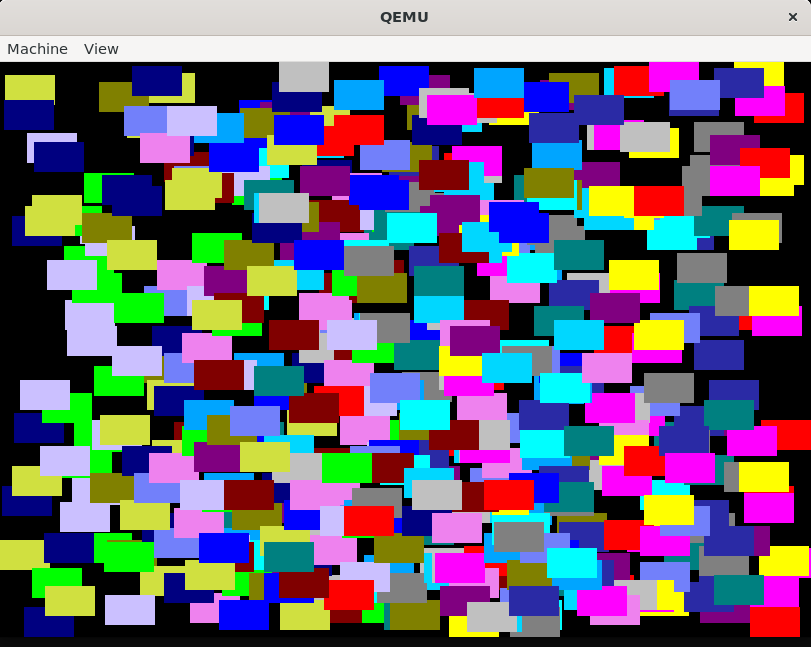
\includegraphics[width=1.0\linewidth]{img/500rechtecke}
  \end{subfigure}
  \caption{Screenshot der Rectangle Demo\\
  500 Rechtecke}
  \label{grafik_2}
\end{figure}


